\setcounter{definition}{0} \setcounter{property}{0} \setcounter{claim}{0} \setcounter{fact}{0} \setcounter{corollary}{0} \setcounter{figure}{0}
\section{RNA Secondary Structure}

A RNA molecule is a chain of nucleotides drawn from $\{A,C,G,U\}$.
Unlike DNA that is double-stranded, in which $A$-$T$ and $G$-$C$ are paired
with hydrogen bonds across the two strands, RNA is single-strand.
To stay at a stable conformation, RNA molecule tends to \emph{fold}
by forming nucleotide-pairs within its single strand.
Such self-pairing structure is called the secondary secondary structure of RNA.

We can observe some properties in RNA secondary structure.
See textbook Algorithm Design~[KT], page 273, for an example.
First, $A$ can only be paired with $U$ and $G$ can only be paired with $C$.
Second, a nucleotide can only be paired with a single nucleotide.
Third, the resulting pairing must be non-crossing~(also called nested).
Formally, if $X[i]$ is paired with $X[j]$, $i < j$, then
nucleotides within $X[i + 1 \cdots j - 1]$ can only be paired within themselves,
i.e., it is not possible to have a pair $X[k]$ with $X[l]$ where $i < k < j$ but $l < i$ or $l > j$.
If a pairing~(a set of pairs) satisfies these 3 constraints, we say it is a valid pairing.
See Figure~\ref{fig:nested}.

\begin{figure}[h]
\centering{

\tikzset{every picture/.style={line width=0.75pt}} %set default line width to 0.75pt        

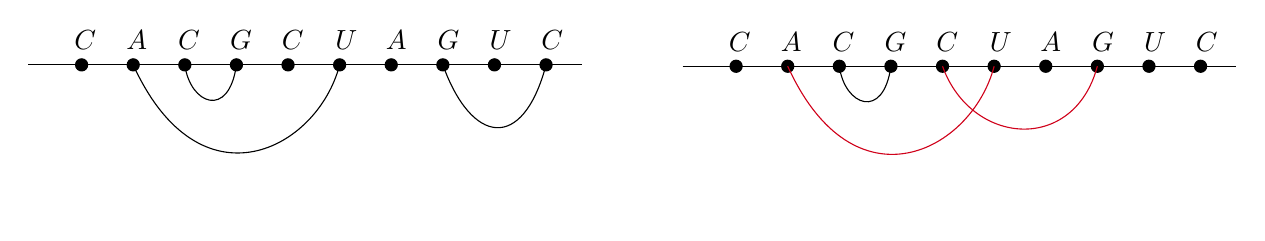
\begin{tikzpicture}[x=0.5pt,y=0.5pt,yscale=-1,xscale=1]
%uncomment if require: \path (0,125); %set diagram left start at 0, and has height of 125

%Flowchart: Connector [id:dp8000065927198341] 
\draw  [fill={rgb, 255:red, 0; green, 0; blue, 0 }  ,fill opacity=1 ] (49,43.9) .. controls (49.87,41.65) and (52.4,40.52) .. (54.66,41.39) .. controls (56.91,42.26) and (58.04,44.79) .. (57.17,47.05) .. controls (56.3,49.3) and (53.77,50.43) .. (51.51,49.56) .. controls (49.26,48.69) and (48.13,46.16) .. (49,43.9) -- cycle ;
%Flowchart: Connector [id:dp15246894411278777] 
\draw  [fill={rgb, 255:red, 0; green, 0; blue, 0 }  ,fill opacity=1 ] (86.3,43.9) .. controls (87.16,41.65) and (89.7,40.52) .. (91.95,41.39) .. controls (94.21,42.26) and (95.33,44.79) .. (94.46,47.05) .. controls (93.59,49.3) and (91.06,50.43) .. (88.81,49.56) .. controls (86.55,48.69) and (85.43,46.16) .. (86.3,43.9) -- cycle ;
%Flowchart: Connector [id:dp36869196941163607] 
\draw  [fill={rgb, 255:red, 0; green, 0; blue, 0 }  ,fill opacity=1 ] (123.59,43.9) .. controls (124.46,41.65) and (126.99,40.52) .. (129.25,41.39) .. controls (131.5,42.26) and (132.63,44.79) .. (131.76,47.05) .. controls (130.89,49.3) and (128.36,50.43) .. (126.1,49.56) .. controls (123.85,48.69) and (122.72,46.16) .. (123.59,43.9) -- cycle ;
%Flowchart: Connector [id:dp16694338209837356] 
\draw  [fill={rgb, 255:red, 0; green, 0; blue, 0 }  ,fill opacity=1 ] (160.89,43.9) .. controls (161.75,41.65) and (164.29,40.52) .. (166.54,41.39) .. controls (168.8,42.26) and (169.92,44.79) .. (169.05,47.05) .. controls (168.18,49.3) and (165.65,50.43) .. (163.4,49.56) .. controls (161.14,48.69) and (160.02,46.16) .. (160.89,43.9) -- cycle ;
%Flowchart: Connector [id:dp42963486447916044] 
\draw  [fill={rgb, 255:red, 0; green, 0; blue, 0 }  ,fill opacity=1 ] (198.18,43.9) .. controls (199.05,41.65) and (201.58,40.52) .. (203.84,41.39) .. controls (206.09,42.26) and (207.22,44.79) .. (206.35,47.05) .. controls (205.48,49.3) and (202.95,50.43) .. (200.69,49.56) .. controls (198.44,48.69) and (197.31,46.16) .. (198.18,43.9) -- cycle ;
%Flowchart: Connector [id:dp5506217339056906] 
\draw  [fill={rgb, 255:red, 0; green, 0; blue, 0 }  ,fill opacity=1 ] (235.48,43.9) .. controls (236.34,41.65) and (238.88,40.52) .. (241.13,41.39) .. controls (243.39,42.26) and (244.51,44.79) .. (243.64,47.05) .. controls (242.77,49.3) and (240.24,50.43) .. (237.99,49.56) .. controls (235.73,48.69) and (234.61,46.16) .. (235.48,43.9) -- cycle ;
%Flowchart: Connector [id:dp9698798449909987] 
\draw  [fill={rgb, 255:red, 0; green, 0; blue, 0 }  ,fill opacity=1 ] (272.77,43.9) .. controls (273.64,41.65) and (276.17,40.52) .. (278.43,41.39) .. controls (280.68,42.26) and (281.81,44.79) .. (280.94,47.05) .. controls (280.07,49.3) and (277.54,50.43) .. (275.28,49.56) .. controls (273.03,48.69) and (271.9,46.16) .. (272.77,43.9) -- cycle ;
%Flowchart: Connector [id:dp6216415603842047] 
\draw  [fill={rgb, 255:red, 0; green, 0; blue, 0 }  ,fill opacity=1 ] (310.07,43.9) .. controls (310.93,41.65) and (313.47,40.52) .. (315.72,41.39) .. controls (317.98,42.26) and (319.1,44.79) .. (318.23,47.05) .. controls (317.36,49.3) and (314.83,50.43) .. (312.58,49.56) .. controls (310.32,48.69) and (309.2,46.16) .. (310.07,43.9) -- cycle ;
%Flowchart: Connector [id:dp3011581402055178] 
\draw  [fill={rgb, 255:red, 0; green, 0; blue, 0 }  ,fill opacity=1 ] (347.36,43.9) .. controls (348.23,41.65) and (350.76,40.52) .. (353.02,41.39) .. controls (355.27,42.26) and (356.4,44.79) .. (355.53,47.05) .. controls (354.66,49.3) and (352.13,50.43) .. (349.87,49.56) .. controls (347.62,48.69) and (346.49,46.16) .. (347.36,43.9) -- cycle ;
%Flowchart: Connector [id:dp9886740109361196] 
\draw  [fill={rgb, 255:red, 0; green, 0; blue, 0 }  ,fill opacity=1 ] (384.66,43.9) .. controls (385.52,41.65) and (388.06,40.52) .. (390.31,41.39) .. controls (392.57,42.26) and (393.69,44.79) .. (392.82,47.05) .. controls (391.95,49.3) and (389.42,50.43) .. (387.17,49.56) .. controls (384.91,48.69) and (383.79,46.16) .. (384.66,43.9) -- cycle ;
%Straight Lines [id:da7380690811587965] 
\draw    (14.5,45.48) -- (414.5,45.48) ;
%Curve Lines [id:da5249448376389138] 
\draw    (90.38,45.48) .. controls (138.5,151) and (223.5,107) .. (239.56,45.48) ;
%Curve Lines [id:da6743430437445295] 
\draw    (127.67,45.48) .. controls (131.5,74) and (159.5,85) .. (164.97,45.48) ;
%Curve Lines [id:da22021299625417579] 
\draw    (314.15,45.48) .. controls (334.8,103) and (371.8,109) .. (388.74,45.48) ;
%Flowchart: Connector [id:dp9581421618036173] 
\draw  [fill={rgb, 255:red, 0; green, 0; blue, 0 }  ,fill opacity=1 ] (522,44.9) .. controls (522.87,42.65) and (525.4,41.52) .. (527.66,42.39) .. controls (529.91,43.26) and (531.04,45.79) .. (530.17,48.05) .. controls (529.3,50.3) and (526.77,51.43) .. (524.51,50.56) .. controls (522.26,49.69) and (521.13,47.16) .. (522,44.9) -- cycle ;
%Flowchart: Connector [id:dp7201955285984009] 
\draw  [fill={rgb, 255:red, 0; green, 0; blue, 0 }  ,fill opacity=1 ] (559.3,44.9) .. controls (560.16,42.65) and (562.7,41.52) .. (564.95,42.39) .. controls (567.21,43.26) and (568.33,45.79) .. (567.46,48.05) .. controls (566.59,50.3) and (564.06,51.43) .. (561.81,50.56) .. controls (559.55,49.69) and (558.43,47.16) .. (559.3,44.9) -- cycle ;
%Flowchart: Connector [id:dp7596225927835101] 
\draw  [fill={rgb, 255:red, 0; green, 0; blue, 0 }  ,fill opacity=1 ] (596.59,44.9) .. controls (597.46,42.65) and (599.99,41.52) .. (602.25,42.39) .. controls (604.5,43.26) and (605.63,45.79) .. (604.76,48.05) .. controls (603.89,50.3) and (601.36,51.43) .. (599.1,50.56) .. controls (596.85,49.69) and (595.72,47.16) .. (596.59,44.9) -- cycle ;
%Flowchart: Connector [id:dp8621287322949679] 
\draw  [fill={rgb, 255:red, 0; green, 0; blue, 0 }  ,fill opacity=1 ] (633.89,44.9) .. controls (634.75,42.65) and (637.29,41.52) .. (639.54,42.39) .. controls (641.8,43.26) and (642.92,45.79) .. (642.05,48.05) .. controls (641.18,50.3) and (638.65,51.43) .. (636.4,50.56) .. controls (634.14,49.69) and (633.02,47.16) .. (633.89,44.9) -- cycle ;
%Flowchart: Connector [id:dp006856865341785978] 
\draw  [fill={rgb, 255:red, 0; green, 0; blue, 0 }  ,fill opacity=1 ] (671.18,44.9) .. controls (672.05,42.65) and (674.58,41.52) .. (676.84,42.39) .. controls (679.09,43.26) and (680.22,45.79) .. (679.35,48.05) .. controls (678.48,50.3) and (675.95,51.43) .. (673.69,50.56) .. controls (671.44,49.69) and (670.31,47.16) .. (671.18,44.9) -- cycle ;
%Flowchart: Connector [id:dp10250658062163487] 
\draw  [fill={rgb, 255:red, 0; green, 0; blue, 0 }  ,fill opacity=1 ] (708.48,44.9) .. controls (709.34,42.65) and (711.88,41.52) .. (714.13,42.39) .. controls (716.39,43.26) and (717.51,45.79) .. (716.64,48.05) .. controls (715.77,50.3) and (713.24,51.43) .. (710.99,50.56) .. controls (708.73,49.69) and (707.61,47.16) .. (708.48,44.9) -- cycle ;
%Flowchart: Connector [id:dp41120137111343924] 
\draw  [fill={rgb, 255:red, 0; green, 0; blue, 0 }  ,fill opacity=1 ] (745.77,44.9) .. controls (746.64,42.65) and (749.17,41.52) .. (751.43,42.39) .. controls (753.68,43.26) and (754.81,45.79) .. (753.94,48.05) .. controls (753.07,50.3) and (750.54,51.43) .. (748.28,50.56) .. controls (746.03,49.69) and (744.9,47.16) .. (745.77,44.9) -- cycle ;
%Flowchart: Connector [id:dp9974209597265988] 
\draw  [fill={rgb, 255:red, 0; green, 0; blue, 0 }  ,fill opacity=1 ] (783.07,44.9) .. controls (783.93,42.65) and (786.47,41.52) .. (788.72,42.39) .. controls (790.98,43.26) and (792.1,45.79) .. (791.23,48.05) .. controls (790.36,50.3) and (787.83,51.43) .. (785.58,50.56) .. controls (783.32,49.69) and (782.2,47.16) .. (783.07,44.9) -- cycle ;
%Flowchart: Connector [id:dp7348756257164472] 
\draw  [fill={rgb, 255:red, 0; green, 0; blue, 0 }  ,fill opacity=1 ] (820.36,44.9) .. controls (821.23,42.65) and (823.76,41.52) .. (826.02,42.39) .. controls (828.27,43.26) and (829.4,45.79) .. (828.53,48.05) .. controls (827.66,50.3) and (825.13,51.43) .. (822.87,50.56) .. controls (820.62,49.69) and (819.49,47.16) .. (820.36,44.9) -- cycle ;
%Flowchart: Connector [id:dp08909097022839452] 
\draw  [fill={rgb, 255:red, 0; green, 0; blue, 0 }  ,fill opacity=1 ] (857.66,44.9) .. controls (858.52,42.65) and (861.06,41.52) .. (863.31,42.39) .. controls (865.57,43.26) and (866.69,45.79) .. (865.82,48.05) .. controls (864.95,50.3) and (862.42,51.43) .. (860.17,50.56) .. controls (857.91,49.69) and (856.79,47.16) .. (857.66,44.9) -- cycle ;
%Straight Lines [id:da05300187439903781] 
\draw    (487.5,46.48) -- (887.5,46.48) ;
%Curve Lines [id:da18802735300363838] 
\draw [color={rgb, 255:red, 208; green, 2; blue, 27 }  ,draw opacity=1 ]   (563.38,46.48) .. controls (611.5,152) and (696.5,108) .. (712.56,46.48) ;
%Curve Lines [id:da12082111624002301] 
\draw    (600.67,46.48) .. controls (604.5,75) and (632.5,86) .. (637.97,46.48) ;
%Curve Lines [id:da8573846720650199] 
\draw [color={rgb, 255:red, 208; green, 2; blue, 27 }  ,draw opacity=1 ]   (675.26,46.48) .. controls (695.91,104) and (770.2,110) .. (787.15,46.48) ;

% Text Node
\draw (46,19) node [anchor=north west][inner sep=0.75pt]   [align=left] {$\displaystyle C$};
% Text Node
\draw (83.5,19) node [anchor=north west][inner sep=0.75pt]   [align=left] {$\displaystyle A$};
% Text Node
\draw (121,19) node [anchor=north west][inner sep=0.75pt]   [align=left] {$\displaystyle C$};
% Text Node
\draw (158.5,19) node [anchor=north west][inner sep=0.75pt]   [align=left] {$\displaystyle G$};
% Text Node
\draw (196,19) node [anchor=north west][inner sep=0.75pt]   [align=left] {$\displaystyle C$};
% Text Node
\draw (234.5,19) node [anchor=north west][inner sep=0.75pt]   [align=left] {$\displaystyle U$};
% Text Node
\draw (271,19) node [anchor=north west][inner sep=0.75pt]   [align=left] {$\displaystyle A$};
% Text Node
\draw (346,19) node [anchor=north west][inner sep=0.75pt]   [align=left] {$\displaystyle U$};
% Text Node
\draw (383.48,19) node [anchor=north west][inner sep=0.75pt]   [align=left] {$\displaystyle C$};
% Text Node
\draw (308.5,19) node [anchor=north west][inner sep=0.75pt]   [align=left] {$\displaystyle G$};
% Text Node
\draw (519,20) node [anchor=north west][inner sep=0.75pt]   [align=left] {$\displaystyle C$};
% Text Node
\draw (556.5,20) node [anchor=north west][inner sep=0.75pt]   [align=left] {$\displaystyle A$};
% Text Node
\draw (594,20) node [anchor=north west][inner sep=0.75pt]   [align=left] {$\displaystyle C$};
% Text Node
\draw (631.5,20) node [anchor=north west][inner sep=0.75pt]   [align=left] {$\displaystyle G$};
% Text Node
\draw (669,20) node [anchor=north west][inner sep=0.75pt]   [align=left] {$\displaystyle C$};
% Text Node
\draw (707.5,20) node [anchor=north west][inner sep=0.75pt]   [align=left] {$\displaystyle U$};
% Text Node
\draw (744,20) node [anchor=north west][inner sep=0.75pt]   [align=left] {$\displaystyle A$};
% Text Node
\draw (819,20) node [anchor=north west][inner sep=0.75pt]   [align=left] {$\displaystyle U$};
% Text Node
\draw (856.48,20) node [anchor=north west][inner sep=0.75pt]   [align=left] {$\displaystyle C$};
% Text Node
\draw (781.5,20) node [anchor=north west][inner sep=0.75pt]   [align=left] {$\displaystyle G$};


\end{tikzpicture}

}
\caption{Left: a valid pairing; Right: a non-valid pairing as the two red pairs cross.}
\label{fig:nested}
\end{figure}

In general, the more pairs a RNA molecule forms, the more stable it will be.
Therefore, ``maximizing pairs'' is a reasonable objective function
in formulating RNA secondary structure problem into an optimization problem.
Formally, given a string $X$ over alphabet $\Sigma = \{A, C, G, U\}$,
we seek a valid pairing of $X$ such that the number of pairs is maximized.

Note: RNA folding is a \emph{science} problem. More factors
are involved and related in
determining its secondary structure, and above description only considers
a subset of these. Even these 3 constraints we described are not always
the case~(exceptions always exist in Biology). The above optimization problem
is a \emph{model} of RNA folding. It's not perfect. In fact, ``all models are wrong''.
``Right'' or ``wrong'' is not the proper criterion in evaluating a model.
As long as a model can explain existing observations, and can predict verifiable outcomes,
it is a \emph{useful} model. After it is formualted as a mathematical problem,
``right'' or ``wrong'' criterion applies: we will design a \emph{correct} algorithm
to solve this formulated problem, and prove that it always returns the optimal solution.

\subsection*{A Dynamic Programming Algorithm}

We again want to design a dynamic programming algorithm.
We first check if it satisfies certain optimal substructure.
See Figure~\ref{fig:optimal}.
Suppose that we know the optimal pairing of $X$,
then its (nested) substructure must be the optimal
pairing of the corresponding substring of $X$.
Formally, let $P$ be an optimal pairing of $X[1\cdots n]$.
If $X[n]$ is not paired in $P$, then we have that
the substructure of $P$ on $X[1\cdots n - 1]$ is an optimal
pairing of $X[1\cdots n - 1]$. (Proof: suppose there exists
a better pairing of $X[1\cdots n - 1]$, then we can concatenate
it with the unpaired $X[n]$ to get a better pairing of $X$.)
If $X[n]$ is paired in $P$, say, with $X[k]$, then we have that
the substructure of $P$ on $X[1\cdots k - 1]$ is an optimal
pairing of $X[1\cdots k - 1]$, and 
the substrcture of $P$ on $X[k + 1\cdots n - 1]$ is an optimal
pairing of $X[k + 1\cdots n - 1]$. 
(Proof: suppose there exists
a better pairing of $X[1\cdots k - 1]$, then we can use it to replace
the coressponding portion of $P$ to 
get a better pairing of $X$. The same for $X[k + 1\cdots n - 1]$.)
An inductive statement leads to that smaller nested substructure
is optimal w.r.t.\ the corresponding substring too~(for example, 
		$ACGCU$, $CGC$, etc, in Figure~\ref{fig:optimal}).

\begin{figure}[h]
\centering{

\tikzset{every picture/.style={line width=0.75pt}} %set default line width to 0.75pt        

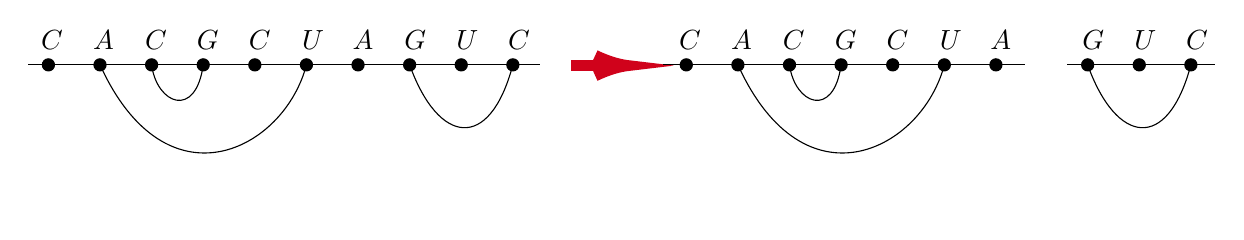
\begin{tikzpicture}[x=0.5pt,y=0.5pt,yscale=-1,xscale=1]
%uncomment if require: \path (0,118); %set diagram left start at 0, and has height of 118

%Flowchart: Connector [id:dp8000065927198341] 
\draw  [fill={rgb, 255:red, 0; green, 0; blue, 0 }  ,fill opacity=1 ] (25,40.9) .. controls (25.87,38.65) and (28.4,37.52) .. (30.66,38.39) .. controls (32.91,39.26) and (34.04,41.79) .. (33.17,44.05) .. controls (32.3,46.3) and (29.77,47.43) .. (27.51,46.56) .. controls (25.26,45.69) and (24.13,43.16) .. (25,40.9) -- cycle ;
%Flowchart: Connector [id:dp15246894411278777] 
\draw  [fill={rgb, 255:red, 0; green, 0; blue, 0 }  ,fill opacity=1 ] (62.3,40.9) .. controls (63.16,38.65) and (65.7,37.52) .. (67.95,38.39) .. controls (70.21,39.26) and (71.33,41.79) .. (70.46,44.05) .. controls (69.59,46.3) and (67.06,47.43) .. (64.81,46.56) .. controls (62.55,45.69) and (61.43,43.16) .. (62.3,40.9) -- cycle ;
%Flowchart: Connector [id:dp36869196941163607] 
\draw  [fill={rgb, 255:red, 0; green, 0; blue, 0 }  ,fill opacity=1 ] (99.59,40.9) .. controls (100.46,38.65) and (102.99,37.52) .. (105.25,38.39) .. controls (107.5,39.26) and (108.63,41.79) .. (107.76,44.05) .. controls (106.89,46.3) and (104.36,47.43) .. (102.1,46.56) .. controls (99.85,45.69) and (98.72,43.16) .. (99.59,40.9) -- cycle ;
%Flowchart: Connector [id:dp16694338209837356] 
\draw  [fill={rgb, 255:red, 0; green, 0; blue, 0 }  ,fill opacity=1 ] (136.89,40.9) .. controls (137.75,38.65) and (140.29,37.52) .. (142.54,38.39) .. controls (144.8,39.26) and (145.92,41.79) .. (145.05,44.05) .. controls (144.18,46.3) and (141.65,47.43) .. (139.4,46.56) .. controls (137.14,45.69) and (136.02,43.16) .. (136.89,40.9) -- cycle ;
%Flowchart: Connector [id:dp42963486447916044] 
\draw  [fill={rgb, 255:red, 0; green, 0; blue, 0 }  ,fill opacity=1 ] (174.18,40.9) .. controls (175.05,38.65) and (177.58,37.52) .. (179.84,38.39) .. controls (182.09,39.26) and (183.22,41.79) .. (182.35,44.05) .. controls (181.48,46.3) and (178.95,47.43) .. (176.69,46.56) .. controls (174.44,45.69) and (173.31,43.16) .. (174.18,40.9) -- cycle ;
%Flowchart: Connector [id:dp5506217339056906] 
\draw  [fill={rgb, 255:red, 0; green, 0; blue, 0 }  ,fill opacity=1 ] (211.48,40.9) .. controls (212.34,38.65) and (214.88,37.52) .. (217.13,38.39) .. controls (219.39,39.26) and (220.51,41.79) .. (219.64,44.05) .. controls (218.77,46.3) and (216.24,47.43) .. (213.99,46.56) .. controls (211.73,45.69) and (210.61,43.16) .. (211.48,40.9) -- cycle ;
%Flowchart: Connector [id:dp9698798449909987] 
\draw  [fill={rgb, 255:red, 0; green, 0; blue, 0 }  ,fill opacity=1 ] (248.77,40.9) .. controls (249.64,38.65) and (252.17,37.52) .. (254.43,38.39) .. controls (256.68,39.26) and (257.81,41.79) .. (256.94,44.05) .. controls (256.07,46.3) and (253.54,47.43) .. (251.28,46.56) .. controls (249.03,45.69) and (247.9,43.16) .. (248.77,40.9) -- cycle ;
%Flowchart: Connector [id:dp6216415603842047] 
\draw  [fill={rgb, 255:red, 0; green, 0; blue, 0 }  ,fill opacity=1 ] (286.07,40.9) .. controls (286.93,38.65) and (289.47,37.52) .. (291.72,38.39) .. controls (293.98,39.26) and (295.1,41.79) .. (294.23,44.05) .. controls (293.36,46.3) and (290.83,47.43) .. (288.58,46.56) .. controls (286.32,45.69) and (285.2,43.16) .. (286.07,40.9) -- cycle ;
%Flowchart: Connector [id:dp3011581402055178] 
\draw  [fill={rgb, 255:red, 0; green, 0; blue, 0 }  ,fill opacity=1 ] (323.36,40.9) .. controls (324.23,38.65) and (326.76,37.52) .. (329.02,38.39) .. controls (331.27,39.26) and (332.4,41.79) .. (331.53,44.05) .. controls (330.66,46.3) and (328.13,47.43) .. (325.87,46.56) .. controls (323.62,45.69) and (322.49,43.16) .. (323.36,40.9) -- cycle ;
%Flowchart: Connector [id:dp9886740109361196] 
\draw  [fill={rgb, 255:red, 0; green, 0; blue, 0 }  ,fill opacity=1 ] (360.66,40.9) .. controls (361.52,38.65) and (364.06,37.52) .. (366.31,38.39) .. controls (368.57,39.26) and (369.69,41.79) .. (368.82,44.05) .. controls (367.95,46.3) and (365.42,47.43) .. (363.17,46.56) .. controls (360.91,45.69) and (359.79,43.16) .. (360.66,40.9) -- cycle ;
%Straight Lines [id:da7380690811587965] 
\draw    (14.5,42.48) -- (384.5,42.48) ;
%Curve Lines [id:da5249448376389138] 
\draw    (66.38,42.48) .. controls (114.5,148) and (199.5,104) .. (215.56,42.48) ;
%Curve Lines [id:da6743430437445295] 
\draw    (103.67,42.48) .. controls (107.5,71) and (135.5,82) .. (140.97,42.48) ;
%Curve Lines [id:da22021299625417579] 
\draw    (290.15,42.48) .. controls (310.8,100) and (347.8,106) .. (364.74,42.48) ;
%Straight Lines [id:da7069209190780016] 
\draw [color={rgb, 255:red, 208; green, 2; blue, 27 }  ,draw opacity=1 ][line width=3.75]    (407,43) -- (443.5,43) ;
\draw [shift={(449.5,43)}, rotate = 180] [color={rgb, 255:red, 208; green, 2; blue, 27 }  ,draw opacity=1 ][line width=3.75]    (25.14,-7.57) .. controls (15.99,-3.21) and (7.61,-0.69) .. (0,0) .. controls (7.61,0.69) and (15.99,3.21) .. (25.14,7.57)   ;
%Flowchart: Connector [id:dp5322197909537895] 
\draw  [fill={rgb, 255:red, 0; green, 0; blue, 0 }  ,fill opacity=1 ] (776.07,40.9) .. controls (776.93,38.65) and (779.47,37.52) .. (781.72,38.39) .. controls (783.98,39.26) and (785.1,41.79) .. (784.23,44.05) .. controls (783.36,46.3) and (780.83,47.43) .. (778.58,46.56) .. controls (776.32,45.69) and (775.2,43.16) .. (776.07,40.9) -- cycle ;
%Flowchart: Connector [id:dp13352675314788975] 
\draw  [fill={rgb, 255:red, 0; green, 0; blue, 0 }  ,fill opacity=1 ] (813.36,40.9) .. controls (814.23,38.65) and (816.76,37.52) .. (819.02,38.39) .. controls (821.27,39.26) and (822.4,41.79) .. (821.53,44.05) .. controls (820.66,46.3) and (818.13,47.43) .. (815.87,46.56) .. controls (813.62,45.69) and (812.49,43.16) .. (813.36,40.9) -- cycle ;
%Flowchart: Connector [id:dp21192888942378674] 
\draw  [fill={rgb, 255:red, 0; green, 0; blue, 0 }  ,fill opacity=1 ] (850.66,40.9) .. controls (851.52,38.65) and (854.06,37.52) .. (856.31,38.39) .. controls (858.57,39.26) and (859.69,41.79) .. (858.82,44.05) .. controls (857.95,46.3) and (855.42,47.43) .. (853.17,46.56) .. controls (850.91,45.69) and (849.79,43.16) .. (850.66,40.9) -- cycle ;
%Straight Lines [id:da824569447163987] 
\draw    (765.5,42.48) -- (872.5,42.48) ;
%Curve Lines [id:da7044902821535391] 
\draw    (780.15,42.48) .. controls (800.8,100) and (837.8,106) .. (854.74,42.48) ;
%Flowchart: Connector [id:dp9350094771084225] 
\draw  [fill={rgb, 255:red, 0; green, 0; blue, 0 }  ,fill opacity=1 ] (486,40.9) .. controls (486.87,38.65) and (489.4,37.52) .. (491.66,38.39) .. controls (493.91,39.26) and (495.04,41.79) .. (494.17,44.05) .. controls (493.3,46.3) and (490.77,47.43) .. (488.51,46.56) .. controls (486.26,45.69) and (485.13,43.16) .. (486,40.9) -- cycle ;
%Flowchart: Connector [id:dp11350907508532626] 
\draw  [fill={rgb, 255:red, 0; green, 0; blue, 0 }  ,fill opacity=1 ] (523.3,40.9) .. controls (524.16,38.65) and (526.7,37.52) .. (528.95,38.39) .. controls (531.21,39.26) and (532.33,41.79) .. (531.46,44.05) .. controls (530.59,46.3) and (528.06,47.43) .. (525.81,46.56) .. controls (523.55,45.69) and (522.43,43.16) .. (523.3,40.9) -- cycle ;
%Flowchart: Connector [id:dp3052785983719639] 
\draw  [fill={rgb, 255:red, 0; green, 0; blue, 0 }  ,fill opacity=1 ] (560.59,40.9) .. controls (561.46,38.65) and (563.99,37.52) .. (566.25,38.39) .. controls (568.5,39.26) and (569.63,41.79) .. (568.76,44.05) .. controls (567.89,46.3) and (565.36,47.43) .. (563.1,46.56) .. controls (560.85,45.69) and (559.72,43.16) .. (560.59,40.9) -- cycle ;
%Flowchart: Connector [id:dp03710718088561116] 
\draw  [fill={rgb, 255:red, 0; green, 0; blue, 0 }  ,fill opacity=1 ] (597.89,40.9) .. controls (598.75,38.65) and (601.29,37.52) .. (603.54,38.39) .. controls (605.8,39.26) and (606.92,41.79) .. (606.05,44.05) .. controls (605.18,46.3) and (602.65,47.43) .. (600.4,46.56) .. controls (598.14,45.69) and (597.02,43.16) .. (597.89,40.9) -- cycle ;
%Flowchart: Connector [id:dp23670841860659286] 
\draw  [fill={rgb, 255:red, 0; green, 0; blue, 0 }  ,fill opacity=1 ] (635.18,40.9) .. controls (636.05,38.65) and (638.58,37.52) .. (640.84,38.39) .. controls (643.09,39.26) and (644.22,41.79) .. (643.35,44.05) .. controls (642.48,46.3) and (639.95,47.43) .. (637.69,46.56) .. controls (635.44,45.69) and (634.31,43.16) .. (635.18,40.9) -- cycle ;
%Flowchart: Connector [id:dp22400416886884278] 
\draw  [fill={rgb, 255:red, 0; green, 0; blue, 0 }  ,fill opacity=1 ] (672.48,40.9) .. controls (673.34,38.65) and (675.88,37.52) .. (678.13,38.39) .. controls (680.39,39.26) and (681.51,41.79) .. (680.64,44.05) .. controls (679.77,46.3) and (677.24,47.43) .. (674.99,46.56) .. controls (672.73,45.69) and (671.61,43.16) .. (672.48,40.9) -- cycle ;
%Flowchart: Connector [id:dp3681462959706371] 
\draw  [fill={rgb, 255:red, 0; green, 0; blue, 0 }  ,fill opacity=1 ] (709.77,40.9) .. controls (710.64,38.65) and (713.17,37.52) .. (715.43,38.39) .. controls (717.68,39.26) and (718.81,41.79) .. (717.94,44.05) .. controls (717.07,46.3) and (714.54,47.43) .. (712.28,46.56) .. controls (710.03,45.69) and (708.9,43.16) .. (709.77,40.9) -- cycle ;
%Straight Lines [id:da2794395954613992] 
\draw    (473.5,42.48) -- (734.5,42.48) ;
%Curve Lines [id:da2506737550157674] 
\draw    (527.38,42.48) .. controls (575.5,148) and (660.5,104) .. (676.56,42.48) ;
%Curve Lines [id:da25133040404462803] 
\draw    (564.67,42.48) .. controls (568.5,71) and (596.5,82) .. (601.97,42.48) ;

% Text Node
\draw (22,16) node [anchor=north west][inner sep=0.75pt]   [align=left] {$\displaystyle C$};
% Text Node
\draw (59.5,16) node [anchor=north west][inner sep=0.75pt]   [align=left] {$\displaystyle A$};
% Text Node
\draw (97,16) node [anchor=north west][inner sep=0.75pt]   [align=left] {$\displaystyle C$};
% Text Node
\draw (134.5,16) node [anchor=north west][inner sep=0.75pt]   [align=left] {$\displaystyle G$};
% Text Node
\draw (172,16) node [anchor=north west][inner sep=0.75pt]   [align=left] {$\displaystyle C$};
% Text Node
\draw (210.5,16) node [anchor=north west][inner sep=0.75pt]   [align=left] {$\displaystyle U$};
% Text Node
\draw (247,16) node [anchor=north west][inner sep=0.75pt]   [align=left] {$\displaystyle A$};
% Text Node
\draw (322,16) node [anchor=north west][inner sep=0.75pt]   [align=left] {$\displaystyle U$};
% Text Node
\draw (359.48,16) node [anchor=north west][inner sep=0.75pt]   [align=left] {$\displaystyle C$};
% Text Node
\draw (284.5,16) node [anchor=north west][inner sep=0.75pt]   [align=left] {$\displaystyle G$};
% Text Node
\draw (812,16) node [anchor=north west][inner sep=0.75pt]   [align=left] {$\displaystyle U$};
% Text Node
\draw (849.48,16) node [anchor=north west][inner sep=0.75pt]   [align=left] {$\displaystyle C$};
% Text Node
\draw (774.5,16) node [anchor=north west][inner sep=0.75pt]   [align=left] {$\displaystyle G$};
% Text Node
\draw (483,16) node [anchor=north west][inner sep=0.75pt]   [align=left] {$\displaystyle C$};
% Text Node
\draw (520.5,16) node [anchor=north west][inner sep=0.75pt]   [align=left] {$\displaystyle A$};
% Text Node
\draw (558,16) node [anchor=north west][inner sep=0.75pt]   [align=left] {$\displaystyle C$};
% Text Node
\draw (595.5,16) node [anchor=north west][inner sep=0.75pt]   [align=left] {$\displaystyle G$};
% Text Node
\draw (633,16) node [anchor=north west][inner sep=0.75pt]   [align=left] {$\displaystyle C$};
% Text Node
\draw (671.5,16) node [anchor=north west][inner sep=0.75pt]   [align=left] {$\displaystyle U$};
% Text Node
\draw (708,16) node [anchor=north west][inner sep=0.75pt]   [align=left] {$\displaystyle A$};


\end{tikzpicture}

}
\caption{Left: an optimal pairing; Middle: an optimal pairing of sustring $ACGCUA$; Right: 
an optimal pairing of substring $GUC$.}
\label{fig:optimal}
\end{figure}

So, this problem indeed satisfies optimal substructure property.
It also suggests defining subproblems \emph{overall substrings}~(or over intervals) of $X$.
Formally, we define $P(i,j)$ as the number of pairs in the optimal pairing of $X[i\cdots j]$.
Clearly, the number of pairs in the optimal pairing of $X$ is $P(1,n)$ where $n = |X|$.

We now develop a recursion, which again is the reverse process of reasoning the optimal substructure
but with necessary enumerations.
See Figure~\ref{fig:recursion}
Specifically, to calculate $P(i,j)$, the optimal pairing over substring $X[i\cdots j]$,
we enumerate all possibilities of the last step, i.e., how $X[j]$ is paired.
The first case is that $X[j]$ is not paired, and in this case $P(i,j) = P(i, j-1)$.
The second case is that $X[j]$ is paired. With whom? We don't know so we enumerate
all possible partner of $X[j]$, which must be one of the $X[k]$ where $i \le k < j$
and that $X[j]$ and $X[k]$ can be paired~(i.e., $A$-$U$ or $G$-$C$).
Once we know that $X[j]$ is paired with $X[k]$, then we have two subproblems
over substrings $X[i\cdots k-1]$ and $X[k + 1 \cdots j - 1]$. Based on above optimal substructure,
these two subproblems must be optimal in order to get the optimal pairing of $X[i\cdots j]$.
Therefore, in this case we have $P(i,j) = \max_{i \le k < j, X[j]\sim X[k] } (1 + P(i, k-1) + P(k+1,j-1))$, where
the extra 1 represents the pair of $(X[k], X[j])$ and I use $X[j]\sim X[k]$ to represent that $X[j]$ and $X[k]$ can be paired.

Combined, we have the following recursion.
\begin{displaymath}
P(i,j) = \max\left\{
	\begin{array}{llll}
	P(i,j-1)\\
	\textstyle \max_{i \le k < j, X[j]\sim X[k]} (1 + P(i,k-1) + P(k+1,j-1)) \\
	\end{array}
\right.
\end{displaymath}

\begin{figure}[h]
\centering{

\tikzset{every picture/.style={line width=0.75pt}} %set default line width to 0.75pt        

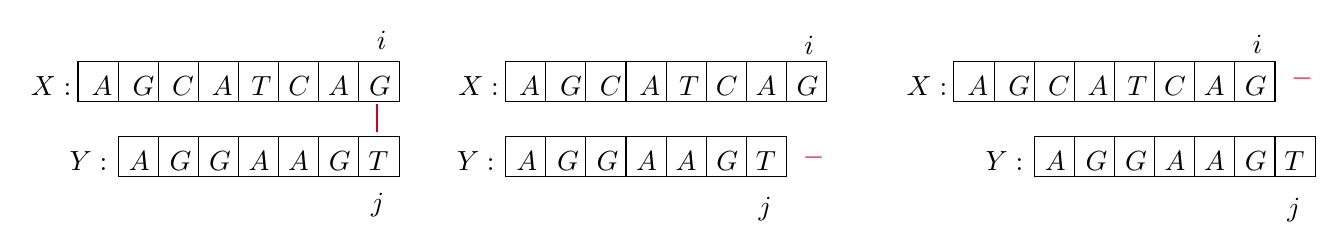
\begin{tikzpicture}[x=0.5pt,y=0.5pt,yscale=-1,xscale=1]
%uncomment if require: \path (0,172); %set diagram left start at 0, and has height of 172

%Straight Lines [id:da5184853822717996] 
\draw [color={rgb, 255:red, 208; green, 2; blue, 27 }  ,draw opacity=1 ][line width=0.75]    (265,71) -- (265,91) ;
%Shape: Grid [id:dp39994906595632274] 
\draw  [draw opacity=0] (49,40) -- (281,40) -- (281,69) -- (49,69) -- cycle ; \draw   (78,40) -- (78,69)(107,40) -- (107,69)(136,40) -- (136,69)(165,40) -- (165,69)(194,40) -- (194,69)(223,40) -- (223,69)(252,40) -- (252,69) ; \draw    ; \draw   (49,40) -- (281,40) -- (281,69) -- (49,69) -- cycle ;
%Shape: Grid [id:dp8100536729244665] 
\draw  [draw opacity=0] (78,94) -- (281,94) -- (281,123) -- (78,123) -- cycle ; \draw   (107,94) -- (107,123)(136,94) -- (136,123)(165,94) -- (165,123)(194,94) -- (194,123)(223,94) -- (223,123)(252,94) -- (252,123) ; \draw    ; \draw   (78,94) -- (281,94) -- (281,123) -- (78,123) -- cycle ;
%Shape: Grid [id:dp4933742529886569] 
\draw  [draw opacity=0] (358,40) -- (590,40) -- (590,69) -- (358,69) -- cycle ; \draw   (387,40) -- (387,69)(416,40) -- (416,69)(445,40) -- (445,69)(474,40) -- (474,69)(503,40) -- (503,69)(532,40) -- (532,69)(561,40) -- (561,69) ; \draw    ; \draw   (358,40) -- (590,40) -- (590,69) -- (358,69) -- cycle ;
%Shape: Grid [id:dp3002745379875943] 
\draw  [draw opacity=0] (358,94) -- (561,94) -- (561,123) -- (358,123) -- cycle ; \draw   (387,94) -- (387,123)(416,94) -- (416,123)(445,94) -- (445,123)(474,94) -- (474,123)(503,94) -- (503,123)(532,94) -- (532,123) ; \draw    ; \draw   (358,94) -- (561,94) -- (561,123) -- (358,123) -- cycle ;
%Shape: Grid [id:dp20349177163511312] 
\draw  [draw opacity=0] (682,40) -- (914,40) -- (914,69) -- (682,69) -- cycle ; \draw   (711,40) -- (711,69)(740,40) -- (740,69)(769,40) -- (769,69)(798,40) -- (798,69)(827,40) -- (827,69)(856,40) -- (856,69)(885,40) -- (885,69) ; \draw    ; \draw   (682,40) -- (914,40) -- (914,69) -- (682,69) -- cycle ;
%Shape: Grid [id:dp02508286059103748] 
\draw  [draw opacity=0] (740,94) -- (943,94) -- (943,123) -- (740,123) -- cycle ; \draw   (769,94) -- (769,123)(798,94) -- (798,123)(827,94) -- (827,123)(856,94) -- (856,123)(885,94) -- (885,123)(914,94) -- (914,123) ; \draw    ; \draw   (740,94) -- (943,94) -- (943,123) -- (740,123) -- cycle ;

% Text Node
\draw (86.5,49) node [anchor=north west][inner sep=0.75pt]   [align=left] {$\displaystyle G$};
% Text Node
\draw (172.45,49) node [anchor=north west][inner sep=0.75pt]   [align=left] {$\displaystyle \textcolor[rgb]{0,0,0}{T}$};
% Text Node
\draw (115.15,49) node [anchor=north west][inner sep=0.75pt]   [align=left] {$\displaystyle C$};
% Text Node
\draw (227.75,49) node [anchor=north west][inner sep=0.75pt]   [align=left] {$\displaystyle A$};
% Text Node
\draw (257.42,49) node [anchor=north west][inner sep=0.75pt]   [align=left] {$\displaystyle G$};
% Text Node
\draw (143.8,49) node [anchor=north west][inner sep=0.75pt]   [align=left] {$\displaystyle A$};
% Text Node
\draw (113.37,103) node [anchor=north west][inner sep=0.75pt]   [align=left] {$\displaystyle G$};
% Text Node
\draw (141.89,103) node [anchor=north west][inner sep=0.75pt]   [align=left] {$\displaystyle G$};
% Text Node
\draw (198.93,103) node [anchor=north west][inner sep=0.75pt]   [align=left] {$\displaystyle A$};
% Text Node
\draw (228.45,103) node [anchor=north west][inner sep=0.75pt]   [align=left] {$\displaystyle G$};
% Text Node
\draw (170.41,103) node [anchor=north west][inner sep=0.75pt]   [align=left] {$\displaystyle A$};
% Text Node
\draw (257,103) node [anchor=north west][inner sep=0.75pt]   [align=left] {$\displaystyle T$};
% Text Node
\draw (56.85,49) node [anchor=north west][inner sep=0.75pt]   [align=left] {$\displaystyle A$};
% Text Node
\draw (83.85,103) node [anchor=north west][inner sep=0.75pt]   [align=left] {$\displaystyle A$};
% Text Node
\draw (199.1,49) node [anchor=north west][inner sep=0.75pt]   [align=left] {$\displaystyle C$};
% Text Node
\draw (13,49) node [anchor=north west][inner sep=0.75pt]   [align=left] {$\displaystyle X:$};
% Text Node
\draw (41,103) node [anchor=north west][inner sep=0.75pt]   [align=left] {$\displaystyle Y:$};
% Text Node
\draw (263,16) node [anchor=north west][inner sep=0.75pt]   [align=left] {$\displaystyle i$};
% Text Node
\draw (259,133) node [anchor=north west][inner sep=0.75pt]   [align=left] {$\displaystyle j$};
% Text Node
\draw (395.5,49) node [anchor=north west][inner sep=0.75pt]   [align=left] {$\displaystyle G$};
% Text Node
\draw (481.45,49) node [anchor=north west][inner sep=0.75pt]   [align=left] {$\displaystyle \textcolor[rgb]{0,0,0}{T}$};
% Text Node
\draw (424.15,49) node [anchor=north west][inner sep=0.75pt]   [align=left] {$\displaystyle C$};
% Text Node
\draw (536.75,49) node [anchor=north west][inner sep=0.75pt]   [align=left] {$\displaystyle A$};
% Text Node
\draw (566.42,49) node [anchor=north west][inner sep=0.75pt]   [align=left] {$\displaystyle G$};
% Text Node
\draw (452.8,49) node [anchor=north west][inner sep=0.75pt]   [align=left] {$\displaystyle A$};
% Text Node
\draw (393.37,103) node [anchor=north west][inner sep=0.75pt]   [align=left] {$\displaystyle G$};
% Text Node
\draw (421.89,103) node [anchor=north west][inner sep=0.75pt]   [align=left] {$\displaystyle G$};
% Text Node
\draw (478.93,103) node [anchor=north west][inner sep=0.75pt]   [align=left] {$\displaystyle A$};
% Text Node
\draw (508.45,103) node [anchor=north west][inner sep=0.75pt]   [align=left] {$\displaystyle G$};
% Text Node
\draw (450.41,103) node [anchor=north west][inner sep=0.75pt]   [align=left] {$\displaystyle A$};
% Text Node
\draw (537,103) node [anchor=north west][inner sep=0.75pt]   [align=left] {$\displaystyle T$};
% Text Node
\draw (365.85,49) node [anchor=north west][inner sep=0.75pt]   [align=left] {$\displaystyle A$};
% Text Node
\draw (363.85,103) node [anchor=north west][inner sep=0.75pt]   [align=left] {$\displaystyle A$};
% Text Node
\draw (508.1,49) node [anchor=north west][inner sep=0.75pt]   [align=left] {$\displaystyle C$};
% Text Node
\draw (322,49) node [anchor=north west][inner sep=0.75pt]   [align=left] {$\displaystyle X:$};
% Text Node
\draw (321,103) node [anchor=north west][inner sep=0.75pt]   [align=left] {$\displaystyle Y:$};
% Text Node
\draw (572,20) node [anchor=north west][inner sep=0.75pt]   [align=left] {$\displaystyle i$};
% Text Node
\draw (539,136) node [anchor=north west][inner sep=0.75pt]   [align=left] {$\displaystyle j$};
% Text Node
\draw (570.93,101) node [anchor=north west][inner sep=0.75pt]   [align=left] {$\displaystyle \textcolor[rgb]{0.82,0.01,0.11}{-}$};
% Text Node
\draw (719.5,49) node [anchor=north west][inner sep=0.75pt]   [align=left] {$\displaystyle G$};
% Text Node
\draw (805.45,49) node [anchor=north west][inner sep=0.75pt]   [align=left] {$\displaystyle \textcolor[rgb]{0,0,0}{T}$};
% Text Node
\draw (748.15,49) node [anchor=north west][inner sep=0.75pt]   [align=left] {$\displaystyle C$};
% Text Node
\draw (860.75,49) node [anchor=north west][inner sep=0.75pt]   [align=left] {$\displaystyle A$};
% Text Node
\draw (890.42,49) node [anchor=north west][inner sep=0.75pt]   [align=left] {$\displaystyle G$};
% Text Node
\draw (776.8,49) node [anchor=north west][inner sep=0.75pt]   [align=left] {$\displaystyle A$};
% Text Node
\draw (775.37,103) node [anchor=north west][inner sep=0.75pt]   [align=left] {$\displaystyle G$};
% Text Node
\draw (803.89,103) node [anchor=north west][inner sep=0.75pt]   [align=left] {$\displaystyle G$};
% Text Node
\draw (860.93,103) node [anchor=north west][inner sep=0.75pt]   [align=left] {$\displaystyle A$};
% Text Node
\draw (890.45,103) node [anchor=north west][inner sep=0.75pt]   [align=left] {$\displaystyle G$};
% Text Node
\draw (832.41,103) node [anchor=north west][inner sep=0.75pt]   [align=left] {$\displaystyle A$};
% Text Node
\draw (919,103) node [anchor=north west][inner sep=0.75pt]   [align=left] {$\displaystyle T$};
% Text Node
\draw (689.85,49) node [anchor=north west][inner sep=0.75pt]   [align=left] {$\displaystyle A$};
% Text Node
\draw (745.85,103) node [anchor=north west][inner sep=0.75pt]   [align=left] {$\displaystyle A$};
% Text Node
\draw (832.1,49) node [anchor=north west][inner sep=0.75pt]   [align=left] {$\displaystyle C$};
% Text Node
\draw (646,49) node [anchor=north west][inner sep=0.75pt]   [align=left] {$\displaystyle X:$};
% Text Node
\draw (703,103) node [anchor=north west][inner sep=0.75pt]   [align=left] {$\displaystyle Y:$};
% Text Node
\draw (896,19) node [anchor=north west][inner sep=0.75pt]   [align=left] {$\displaystyle i$};
% Text Node
\draw (921,137) node [anchor=north west][inner sep=0.75pt]   [align=left] {$\displaystyle j$};
% Text Node
\draw (923.93,44) node [anchor=north west][inner sep=0.75pt]   [align=left] {$\displaystyle \textcolor[rgb]{0.82,0.01,0.11}{-}$};


\end{tikzpicture}

}
\caption{Two cases in developing the recursion.}
\label{fig:recursion}
\end{figure}


We now complete the algorithm by filling the DP table.
Note that for this problem we \emph{cannot} fill the table row-by-row with increasing row-index.
See Figure~\ref{fig:table}.
This is because, the the calculation of $P(i,j)$ relies on subproblems $P(k + 1, j - 1)$ where $k \ge i$.
A feasible way is to fill the table following the diagnals.
This is essentially to solve subproblems in increasing order of the length of the substrings, i.e.,
first solving substrings of length 1~(i.e., $(X[i], X[i])$, $1\le i \le n$), 
then solving substrings of length 2~(i.e., $(X[i], X[i + 1])$, $1\le i \le n - 1$), 
then solving substrings of length 3~(i.e., $(X[i], X[i + 2])$, $1\le i \le n - 2$),
and so on. 

\begin{figure}[h]
\centering{

\tikzset{every picture/.style={line width=0.75pt}} %set default line width to 0.75pt        

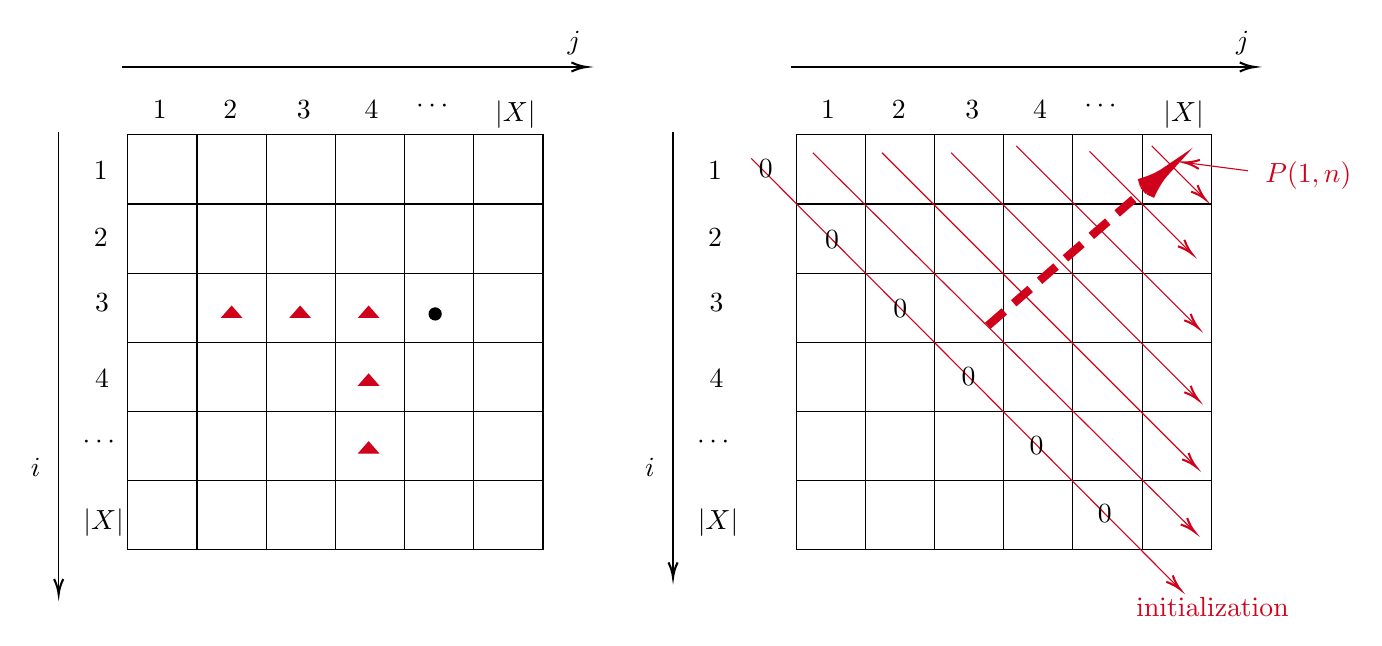
\begin{tikzpicture}[x=0.5pt,y=0.5pt,yscale=-1,xscale=1]
%uncomment if require: \path (0,447); %set diagram left start at 0, and has height of 447

%Shape: Grid [id:dp9095284515127875] 
\draw  [draw opacity=0] (87,90) -- (387,90) -- (387,390) -- (87,390) -- cycle ; \draw   (137,90) -- (137,390)(187,90) -- (187,390)(237,90) -- (237,390)(287,90) -- (287,390)(337,90) -- (337,390) ; \draw   (87,140) -- (387,140)(87,190) -- (387,190)(87,240) -- (387,240)(87,290) -- (387,290)(87,340) -- (387,340) ; \draw   (87,90) -- (387,90) -- (387,390) -- (87,390) -- cycle ;
%Straight Lines [id:da5347307434268296] 
\draw    (37,88) -- (37,420) ;
\draw [shift={(37,422)}, rotate = 270] [color={rgb, 255:red, 0; green, 0; blue, 0 }  ][line width=0.75]    (10.93,-3.29) .. controls (6.95,-1.4) and (3.31,-0.3) .. (0,0) .. controls (3.31,0.3) and (6.95,1.4) .. (10.93,3.29)   ;
%Straight Lines [id:da4989887299865372] 
\draw    (83,41) -- (416.5,41) ;
\draw [shift={(418.5,41)}, rotate = 180] [color={rgb, 255:red, 0; green, 0; blue, 0 }  ][line width=0.75]    (10.93,-3.29) .. controls (6.95,-1.4) and (3.31,-0.3) .. (0,0) .. controls (3.31,0.3) and (6.95,1.4) .. (10.93,3.29)   ;
%Flowchart: Connector [id:dp07878936208838816] 
\draw  [fill={rgb, 255:red, 0; green, 0; blue, 0 }  ,fill opacity=1 ] (305,217.9) .. controls (305.87,215.65) and (308.4,214.52) .. (310.66,215.39) .. controls (312.91,216.26) and (314.04,218.79) .. (313.17,221.05) .. controls (312.3,223.3) and (309.77,224.43) .. (307.51,223.56) .. controls (305.26,222.69) and (304.13,220.16) .. (305,217.9) -- cycle ;
%Shape: Triangle [id:dp6109876057002935] 
\draw  [color={rgb, 255:red, 208; green, 2; blue, 27 }  ,draw opacity=1 ][fill={rgb, 255:red, 208; green, 2; blue, 27 }  ,fill opacity=1 ] (261,214) -- (268,222) -- (254,222) -- cycle ;
%Shape: Triangle [id:dp003677095504452388] 
\draw  [color={rgb, 255:red, 208; green, 2; blue, 27 }  ,draw opacity=1 ][fill={rgb, 255:red, 208; green, 2; blue, 27 }  ,fill opacity=1 ] (211.5,214) -- (218.5,222) -- (204.5,222) -- cycle ;
%Shape: Triangle [id:dp543232883301439] 
\draw  [color={rgb, 255:red, 208; green, 2; blue, 27 }  ,draw opacity=1 ][fill={rgb, 255:red, 208; green, 2; blue, 27 }  ,fill opacity=1 ] (162,214) -- (169,222) -- (155,222) -- cycle ;
%Shape: Triangle [id:dp29900180690969524] 
\draw  [color={rgb, 255:red, 208; green, 2; blue, 27 }  ,draw opacity=1 ][fill={rgb, 255:red, 208; green, 2; blue, 27 }  ,fill opacity=1 ] (261,263) -- (268,271) -- (254,271) -- cycle ;
%Shape: Triangle [id:dp5517868734647194] 
\draw  [color={rgb, 255:red, 208; green, 2; blue, 27 }  ,draw opacity=1 ][fill={rgb, 255:red, 208; green, 2; blue, 27 }  ,fill opacity=1 ] (261,312) -- (268,320) -- (254,320) -- cycle ;
%Shape: Grid [id:dp8676217076414684] 
\draw  [draw opacity=0] (570,90) -- (870,90) -- (870,390) -- (570,390) -- cycle ; \draw   (620,90) -- (620,390)(670,90) -- (670,390)(720,90) -- (720,390)(770,90) -- (770,390)(820,90) -- (820,390) ; \draw   (570,140) -- (870,140)(570,190) -- (870,190)(570,240) -- (870,240)(570,290) -- (870,290)(570,340) -- (870,340) ; \draw   (570,90) -- (870,90) -- (870,390) -- (570,390) -- cycle ;
%Straight Lines [id:da23917339503157053] 
\draw    (481,88) -- (481,408) ;
\draw [shift={(481,410)}, rotate = 270] [color={rgb, 255:red, 0; green, 0; blue, 0 }  ][line width=0.75]    (10.93,-3.29) .. controls (6.95,-1.4) and (3.31,-0.3) .. (0,0) .. controls (3.31,0.3) and (6.95,1.4) .. (10.93,3.29)   ;
%Straight Lines [id:da1200250503088851] 
\draw    (566,41) -- (899.5,41) ;
\draw [shift={(901.5,41)}, rotate = 180] [color={rgb, 255:red, 0; green, 0; blue, 0 }  ][line width=0.75]    (10.93,-3.29) .. controls (6.95,-1.4) and (3.31,-0.3) .. (0,0) .. controls (3.31,0.3) and (6.95,1.4) .. (10.93,3.29)   ;
%Straight Lines [id:da5849775638339646] 
\draw [color={rgb, 255:red, 208; green, 2; blue, 27 }  ,draw opacity=1 ]   (896.5,116) -- (852.48,110.26) ;
\draw [shift={(850.5,110)}, rotate = 367.43] [color={rgb, 255:red, 208; green, 2; blue, 27 }  ,draw opacity=1 ][line width=0.75]    (10.93,-3.29) .. controls (6.95,-1.4) and (3.31,-0.3) .. (0,0) .. controls (3.31,0.3) and (6.95,1.4) .. (10.93,3.29)   ;
%Straight Lines [id:da7158674315801672] 
\draw [color={rgb, 255:red, 208; green, 2; blue, 27 }  ,draw opacity=1 ]   (537.5,107) -- (846.09,417.08) ;
\draw [shift={(847.5,418.5)}, rotate = 225.14] [color={rgb, 255:red, 208; green, 2; blue, 27 }  ,draw opacity=1 ][line width=0.75]    (10.93,-3.29) .. controls (6.95,-1.4) and (3.31,-0.3) .. (0,0) .. controls (3.31,0.3) and (6.95,1.4) .. (10.93,3.29)   ;
%Straight Lines [id:da06318163354731099] 
\draw [color={rgb, 255:red, 208; green, 2; blue, 27 }  ,draw opacity=1 ]   (582,103) -- (856.58,375.59) ;
\draw [shift={(858,377)}, rotate = 224.79] [color={rgb, 255:red, 208; green, 2; blue, 27 }  ,draw opacity=1 ][line width=0.75]    (10.93,-3.29) .. controls (6.95,-1.4) and (3.31,-0.3) .. (0,0) .. controls (3.31,0.3) and (6.95,1.4) .. (10.93,3.29)   ;
%Straight Lines [id:da7422545951430948] 
\draw [color={rgb, 255:red, 208; green, 2; blue, 27 }  ,draw opacity=1 ]   (632,103) -- (857.59,328.59) ;
\draw [shift={(859,330)}, rotate = 225] [color={rgb, 255:red, 208; green, 2; blue, 27 }  ,draw opacity=1 ][line width=0.75]    (10.93,-3.29) .. controls (6.95,-1.4) and (3.31,-0.3) .. (0,0) .. controls (3.31,0.3) and (6.95,1.4) .. (10.93,3.29)   ;
%Straight Lines [id:da6389984033381221] 
\draw [color={rgb, 255:red, 208; green, 2; blue, 27 }  ,draw opacity=1 ]   (682,103) -- (859.09,280.09) ;
\draw [shift={(860.5,281.5)}, rotate = 225] [color={rgb, 255:red, 208; green, 2; blue, 27 }  ,draw opacity=1 ][line width=0.75]    (10.93,-3.29) .. controls (6.95,-1.4) and (3.31,-0.3) .. (0,0) .. controls (3.31,0.3) and (6.95,1.4) .. (10.93,3.29)   ;
%Straight Lines [id:da7613617756284687] 
\draw [color={rgb, 255:red, 208; green, 2; blue, 27 }  ,draw opacity=1 ]   (729,98) -- (859.09,228.09) ;
\draw [shift={(860.5,229.5)}, rotate = 225] [color={rgb, 255:red, 208; green, 2; blue, 27 }  ,draw opacity=1 ][line width=0.75]    (10.93,-3.29) .. controls (6.95,-1.4) and (3.31,-0.3) .. (0,0) .. controls (3.31,0.3) and (6.95,1.4) .. (10.93,3.29)   ;
%Straight Lines [id:da7035765059521567] 
\draw [color={rgb, 255:red, 208; green, 2; blue, 27 }  ,draw opacity=1 ]   (782,102) -- (854.59,174.59) ;
\draw [shift={(856,176)}, rotate = 225] [color={rgb, 255:red, 208; green, 2; blue, 27 }  ,draw opacity=1 ][line width=0.75]    (10.93,-3.29) .. controls (6.95,-1.4) and (3.31,-0.3) .. (0,0) .. controls (3.31,0.3) and (6.95,1.4) .. (10.93,3.29)   ;
%Straight Lines [id:da156242521236438] 
\draw [color={rgb, 255:red, 208; green, 2; blue, 27 }  ,draw opacity=1 ]   (827,98) -- (864.09,135.09) ;
\draw [shift={(865.5,136.5)}, rotate = 225] [color={rgb, 255:red, 208; green, 2; blue, 27 }  ,draw opacity=1 ][line width=0.75]    (10.93,-3.29) .. controls (6.95,-1.4) and (3.31,-0.3) .. (0,0) .. controls (3.31,0.3) and (6.95,1.4) .. (10.93,3.29)   ;
%Straight Lines [id:da421849353700268] 
\draw [color={rgb, 255:red, 208; green, 2; blue, 27 }  ,draw opacity=1 ][line width=3]  [dash pattern={on 7.88pt off 4.5pt}]  (708.5,228) -- (833.72,119.28) ;
\draw [shift={(837.5,116)}, rotate = 499.03] [color={rgb, 255:red, 208; green, 2; blue, 27 }  ,draw opacity=1 ][line width=3]    (20.77,-6.25) .. controls (13.2,-2.65) and (6.28,-0.57) .. (0,0) .. controls (6.28,0.57) and (13.2,2.66) .. (20.77,6.25)   ;

% Text Node
\draw (68,103) node [anchor=north west][inner sep=0.75pt]   [align=left] {$ $};
% Text Node
\draw (60.5,107.38) node [anchor=north west][inner sep=0.75pt]   [align=left] {$\displaystyle 1$};
% Text Node
\draw (52.5,306.14) node [anchor=north west][inner sep=0.75pt]   [align=left] {$\displaystyle \cdots $};
% Text Node
\draw (15,322) node [anchor=north west][inner sep=0.75pt]   [align=left] {$\displaystyle i$};
% Text Node
\draw (403,13) node [anchor=north west][inner sep=0.75pt]   [align=left] {$\displaystyle j$};
% Text Node
\draw (293.4,63.44) node [anchor=north west][inner sep=0.75pt]   [align=left] {$\displaystyle \cdots $};
% Text Node
\draw (60.5,155.76) node [anchor=north west][inner sep=0.75pt]   [align=left] {$\displaystyle 2$};
% Text Node
\draw (103.1,63.44) node [anchor=north west][inner sep=0.75pt]   [align=left] {$\displaystyle 1$};
% Text Node
\draw (154.2,63.44) node [anchor=north west][inner sep=0.75pt]   [align=left] {$\displaystyle 2$};
% Text Node
\draw (350.5,63.44) node [anchor=north west][inner sep=0.75pt]   [align=left] {$\displaystyle | X|$};
% Text Node
\draw (207.3,63.44) node [anchor=north west][inner sep=0.75pt]   [align=left] {$\displaystyle 3$};
% Text Node
\draw (53,358.5) node [anchor=north west][inner sep=0.75pt]   [align=left] {$\displaystyle | X|$};
% Text Node
\draw (61.5,202.76) node [anchor=north west][inner sep=0.75pt]   [align=left] {$\displaystyle 3$};
% Text Node
\draw (61.5,257.76) node [anchor=north west][inner sep=0.75pt]   [align=left] {$\displaystyle 4$};
% Text Node
\draw (256.3,63.44) node [anchor=north west][inner sep=0.75pt]   [align=left] {$\displaystyle 4$};
% Text Node
\draw (512,103) node [anchor=north west][inner sep=0.75pt]   [align=left] {$ $};
% Text Node
\draw (504.5,107.38) node [anchor=north west][inner sep=0.75pt]   [align=left] {$\displaystyle 1$};
% Text Node
\draw (496.5,306.14) node [anchor=north west][inner sep=0.75pt]   [align=left] {$\displaystyle \cdots $};
% Text Node
\draw (459,322) node [anchor=north west][inner sep=0.75pt]   [align=left] {$\displaystyle i$};
% Text Node
\draw (886,13) node [anchor=north west][inner sep=0.75pt]   [align=left] {$\displaystyle j$};
% Text Node
\draw (776.4,63.44) node [anchor=north west][inner sep=0.75pt]   [align=left] {$\displaystyle \cdots $};
% Text Node
\draw (504.5,155.76) node [anchor=north west][inner sep=0.75pt]   [align=left] {$\displaystyle 2$};
% Text Node
\draw (586.1,63.44) node [anchor=north west][inner sep=0.75pt]   [align=left] {$\displaystyle 1$};
% Text Node
\draw (637.2,63.44) node [anchor=north west][inner sep=0.75pt]   [align=left] {$\displaystyle 2$};
% Text Node
\draw (833.5,63.44) node [anchor=north west][inner sep=0.75pt]   [align=left] {$\displaystyle | X|$};
% Text Node
\draw (690.3,63.44) node [anchor=north west][inner sep=0.75pt]   [align=left] {$\displaystyle 3$};
% Text Node
\draw (907.2,107.44) node [anchor=north west][inner sep=0.75pt]   [align=left] {$\displaystyle \textcolor[rgb]{0.82,0.01,0.11}{P}\textcolor[rgb]{0.82,0.01,0.11}{(}\textcolor[rgb]{0.82,0.01,0.11}{1,n}\textcolor[rgb]{0.82,0.01,0.11}{)}$};
% Text Node
\draw (497,358.5) node [anchor=north west][inner sep=0.75pt]   [align=left] {$\displaystyle | X|$};
% Text Node
\draw (505.5,202.76) node [anchor=north west][inner sep=0.75pt]   [align=left] {$\displaystyle 3$};
% Text Node
\draw (505.5,257.76) node [anchor=north west][inner sep=0.75pt]   [align=left] {$\displaystyle 4$};
% Text Node
\draw (739.3,63.44) node [anchor=north west][inner sep=0.75pt]   [align=left] {$\displaystyle 4$};
% Text Node
\draw (589.1,157.44) node [anchor=north west][inner sep=0.75pt]   [align=left] {$\displaystyle 0$};
% Text Node
\draw (638.35,206.94) node [anchor=north west][inner sep=0.75pt]   [align=left] {$\displaystyle 0$};
% Text Node
\draw (687.6,256.44) node [anchor=north west][inner sep=0.75pt]   [align=left] {$\displaystyle 0$};
% Text Node
\draw (736.85,305.94) node [anchor=north west][inner sep=0.75pt]   [align=left] {$\displaystyle 0$};
% Text Node
\draw (786.1,355.44) node [anchor=north west][inner sep=0.75pt]   [align=left] {$\displaystyle 0$};
% Text Node
\draw (814,422) node [anchor=north west][inner sep=0.75pt]   [align=left] {\textcolor[rgb]{0.82,0.01,0.11}{initialization}};
% Text Node
\draw (541.1,106.44) node [anchor=north west][inner sep=0.75pt]   [align=left] {$\displaystyle 0$};


\end{tikzpicture}

}
\caption{Left: the DP table showing the entries~(in red triangles) needed by the current entry~(in black dot).
Right: the order to fill the table.}
\label{fig:table}
\end{figure}

The pseudo-code is given below. 
To faciliate applying the recursion, we initialize $P(i, i - 1) = 0$, $1 \le i \le n$.
We define variable $d = j - i + 1$ to represent the length of substring and use it to index the outer loop; in this way,
we are examining substrings with increasing length.
We use variable $i$ to locate the starting position of each substring.
Once $d$ and $i$ are fixed, the ending position of the substring $j$ will be $i + d - 1$.
The running time of this algorithm is $O(n^3)$, as the calculation
of each entry takes $O(n)$ time.

\begin{minipage}{0.8\textwidth}
	\aaA {14}{Algorithm rna-folding~(string $X$ of length $n$)}\xxx
	\aab {$P(i,i-1) = 0$, for any $1 \le i \le n$}\xxx
	\aaB {10}{for $d = 1 \to n$}\xxx
	\aaC {8}{for $i = 1 \to n-d+1$}\xxx
	\aad {$j = i + d -1$;}\xxx
	\aad {$P(i,j) = P(i, j - 1)$;}\xxx
	\aaD {4}{for $k = i \to j - 1$}\xxx
	\aaE {2}{if~($X[k]$ and $X[j]$ can be paired, and $P(i,j) < P(i,k-1) + P(k+1,j-1) + 1$);}\xxx
	\aaf {$P(i,j) = P(i,k-1) + P(k+1,j-1) + 1$;}\xxx
	\aae {end if;}\xxx
	\aad {end for;}\xxx
	\aac {end for;}\xxx
	\aab {end for;}\xxx
	\aab {report: $P(1,n)$;}\xxx
	\aaa {end algorithm;}\xxx
\end{minipage}


